% Options for packages loaded elsewhere
\PassOptionsToPackage{unicode}{hyperref}
\PassOptionsToPackage{hyphens}{url}
\PassOptionsToPackage{dvipsnames,svgnames,x11names}{xcolor}
%
\documentclass[
  letterpaper,
  DIV=11,
  numbers=noendperiod]{scrreprt}

\usepackage{amsmath,amssymb}
\usepackage{iftex}
\ifPDFTeX
  \usepackage[T1]{fontenc}
  \usepackage[utf8]{inputenc}
  \usepackage{textcomp} % provide euro and other symbols
\else % if luatex or xetex
  \usepackage{unicode-math}
  \defaultfontfeatures{Scale=MatchLowercase}
  \defaultfontfeatures[\rmfamily]{Ligatures=TeX,Scale=1}
\fi
\usepackage{lmodern}
\ifPDFTeX\else  
    % xetex/luatex font selection
\fi
% Use upquote if available, for straight quotes in verbatim environments
\IfFileExists{upquote.sty}{\usepackage{upquote}}{}
\IfFileExists{microtype.sty}{% use microtype if available
  \usepackage[]{microtype}
  \UseMicrotypeSet[protrusion]{basicmath} % disable protrusion for tt fonts
}{}
\makeatletter
\@ifundefined{KOMAClassName}{% if non-KOMA class
  \IfFileExists{parskip.sty}{%
    \usepackage{parskip}
  }{% else
    \setlength{\parindent}{0pt}
    \setlength{\parskip}{6pt plus 2pt minus 1pt}}
}{% if KOMA class
  \KOMAoptions{parskip=half}}
\makeatother
\usepackage{xcolor}
\setlength{\emergencystretch}{3em} % prevent overfull lines
\setcounter{secnumdepth}{-\maxdimen} % remove section numbering
% Make \paragraph and \subparagraph free-standing
\makeatletter
\ifx\paragraph\undefined\else
  \let\oldparagraph\paragraph
  \renewcommand{\paragraph}{
    \@ifstar
      \xxxParagraphStar
      \xxxParagraphNoStar
  }
  \newcommand{\xxxParagraphStar}[1]{\oldparagraph*{#1}\mbox{}}
  \newcommand{\xxxParagraphNoStar}[1]{\oldparagraph{#1}\mbox{}}
\fi
\ifx\subparagraph\undefined\else
  \let\oldsubparagraph\subparagraph
  \renewcommand{\subparagraph}{
    \@ifstar
      \xxxSubParagraphStar
      \xxxSubParagraphNoStar
  }
  \newcommand{\xxxSubParagraphStar}[1]{\oldsubparagraph*{#1}\mbox{}}
  \newcommand{\xxxSubParagraphNoStar}[1]{\oldsubparagraph{#1}\mbox{}}
\fi
\makeatother

\usepackage{color}
\usepackage{fancyvrb}
\newcommand{\VerbBar}{|}
\newcommand{\VERB}{\Verb[commandchars=\\\{\}]}
\DefineVerbatimEnvironment{Highlighting}{Verbatim}{commandchars=\\\{\}}
% Add ',fontsize=\small' for more characters per line
\usepackage{framed}
\definecolor{shadecolor}{RGB}{241,243,245}
\newenvironment{Shaded}{\begin{snugshade}}{\end{snugshade}}
\newcommand{\AlertTok}[1]{\textcolor[rgb]{0.68,0.00,0.00}{#1}}
\newcommand{\AnnotationTok}[1]{\textcolor[rgb]{0.37,0.37,0.37}{#1}}
\newcommand{\AttributeTok}[1]{\textcolor[rgb]{0.40,0.45,0.13}{#1}}
\newcommand{\BaseNTok}[1]{\textcolor[rgb]{0.68,0.00,0.00}{#1}}
\newcommand{\BuiltInTok}[1]{\textcolor[rgb]{0.00,0.23,0.31}{#1}}
\newcommand{\CharTok}[1]{\textcolor[rgb]{0.13,0.47,0.30}{#1}}
\newcommand{\CommentTok}[1]{\textcolor[rgb]{0.37,0.37,0.37}{#1}}
\newcommand{\CommentVarTok}[1]{\textcolor[rgb]{0.37,0.37,0.37}{\textit{#1}}}
\newcommand{\ConstantTok}[1]{\textcolor[rgb]{0.56,0.35,0.01}{#1}}
\newcommand{\ControlFlowTok}[1]{\textcolor[rgb]{0.00,0.23,0.31}{\textbf{#1}}}
\newcommand{\DataTypeTok}[1]{\textcolor[rgb]{0.68,0.00,0.00}{#1}}
\newcommand{\DecValTok}[1]{\textcolor[rgb]{0.68,0.00,0.00}{#1}}
\newcommand{\DocumentationTok}[1]{\textcolor[rgb]{0.37,0.37,0.37}{\textit{#1}}}
\newcommand{\ErrorTok}[1]{\textcolor[rgb]{0.68,0.00,0.00}{#1}}
\newcommand{\ExtensionTok}[1]{\textcolor[rgb]{0.00,0.23,0.31}{#1}}
\newcommand{\FloatTok}[1]{\textcolor[rgb]{0.68,0.00,0.00}{#1}}
\newcommand{\FunctionTok}[1]{\textcolor[rgb]{0.28,0.35,0.67}{#1}}
\newcommand{\ImportTok}[1]{\textcolor[rgb]{0.00,0.46,0.62}{#1}}
\newcommand{\InformationTok}[1]{\textcolor[rgb]{0.37,0.37,0.37}{#1}}
\newcommand{\KeywordTok}[1]{\textcolor[rgb]{0.00,0.23,0.31}{\textbf{#1}}}
\newcommand{\NormalTok}[1]{\textcolor[rgb]{0.00,0.23,0.31}{#1}}
\newcommand{\OperatorTok}[1]{\textcolor[rgb]{0.37,0.37,0.37}{#1}}
\newcommand{\OtherTok}[1]{\textcolor[rgb]{0.00,0.23,0.31}{#1}}
\newcommand{\PreprocessorTok}[1]{\textcolor[rgb]{0.68,0.00,0.00}{#1}}
\newcommand{\RegionMarkerTok}[1]{\textcolor[rgb]{0.00,0.23,0.31}{#1}}
\newcommand{\SpecialCharTok}[1]{\textcolor[rgb]{0.37,0.37,0.37}{#1}}
\newcommand{\SpecialStringTok}[1]{\textcolor[rgb]{0.13,0.47,0.30}{#1}}
\newcommand{\StringTok}[1]{\textcolor[rgb]{0.13,0.47,0.30}{#1}}
\newcommand{\VariableTok}[1]{\textcolor[rgb]{0.07,0.07,0.07}{#1}}
\newcommand{\VerbatimStringTok}[1]{\textcolor[rgb]{0.13,0.47,0.30}{#1}}
\newcommand{\WarningTok}[1]{\textcolor[rgb]{0.37,0.37,0.37}{\textit{#1}}}

\providecommand{\tightlist}{%
  \setlength{\itemsep}{0pt}\setlength{\parskip}{0pt}}\usepackage{longtable,booktabs,array}
\usepackage{calc} % for calculating minipage widths
% Correct order of tables after \paragraph or \subparagraph
\usepackage{etoolbox}
\makeatletter
\patchcmd\longtable{\par}{\if@noskipsec\mbox{}\fi\par}{}{}
\makeatother
% Allow footnotes in longtable head/foot
\IfFileExists{footnotehyper.sty}{\usepackage{footnotehyper}}{\usepackage{footnote}}
\makesavenoteenv{longtable}
\usepackage{graphicx}
\makeatletter
\newsavebox\pandoc@box
\newcommand*\pandocbounded[1]{% scales image to fit in text height/width
  \sbox\pandoc@box{#1}%
  \Gscale@div\@tempa{\textheight}{\dimexpr\ht\pandoc@box+\dp\pandoc@box\relax}%
  \Gscale@div\@tempb{\linewidth}{\wd\pandoc@box}%
  \ifdim\@tempb\p@<\@tempa\p@\let\@tempa\@tempb\fi% select the smaller of both
  \ifdim\@tempa\p@<\p@\scalebox{\@tempa}{\usebox\pandoc@box}%
  \else\usebox{\pandoc@box}%
  \fi%
}
% Set default figure placement to htbp
\def\fps@figure{htbp}
\makeatother

\KOMAoption{captions}{tableheading}
\makeatletter
\@ifpackageloaded{caption}{}{\usepackage{caption}}
\AtBeginDocument{%
\ifdefined\contentsname
  \renewcommand*\contentsname{Table of contents}
\else
  \newcommand\contentsname{Table of contents}
\fi
\ifdefined\listfigurename
  \renewcommand*\listfigurename{List of Figures}
\else
  \newcommand\listfigurename{List of Figures}
\fi
\ifdefined\listtablename
  \renewcommand*\listtablename{List of Tables}
\else
  \newcommand\listtablename{List of Tables}
\fi
\ifdefined\figurename
  \renewcommand*\figurename{Figure}
\else
  \newcommand\figurename{Figure}
\fi
\ifdefined\tablename
  \renewcommand*\tablename{Table}
\else
  \newcommand\tablename{Table}
\fi
}
\@ifpackageloaded{float}{}{\usepackage{float}}
\floatstyle{ruled}
\@ifundefined{c@chapter}{\newfloat{codelisting}{h}{lop}}{\newfloat{codelisting}{h}{lop}[chapter]}
\floatname{codelisting}{Listing}
\newcommand*\listoflistings{\listof{codelisting}{List of Listings}}
\makeatother
\makeatletter
\makeatother
\makeatletter
\@ifpackageloaded{caption}{}{\usepackage{caption}}
\@ifpackageloaded{subcaption}{}{\usepackage{subcaption}}
\makeatother

\usepackage{bookmark}

\IfFileExists{xurl.sty}{\usepackage{xurl}}{} % add URL line breaks if available
\urlstyle{same} % disable monospaced font for URLs
\hypersetup{
  colorlinks=true,
  linkcolor={blue},
  filecolor={Maroon},
  citecolor={Blue},
  urlcolor={Blue},
  pdfcreator={LaTeX via pandoc}}


\author{}
\date{}

\begin{document}


\chapter{Hypothesis Testing}\label{hypothesis-testing}

\section*{Slides}\label{slides}
\addcontentsline{toc}{section}{Slides}

Chapter slides \href{chap2.html}{here}. (To convert html to pdf, press E
\(\to\) Print \(\to\) Destination: Save to pdf)

\section*{R code}\label{r-code}
\addcontentsline{toc}{section}{R code}

\begin{Shaded}
\begin{Highlighting}[]
\DocumentationTok{\#\#\#\#\#\#\#\#\#\#\#\#\#\#\#\#\#\#\#\#\#\#\#\#\#\#\#\#\#\#\#\#\#\#\#\#\#\#\#\#\#\#\#\#\#\#\#\#\#\#\#\#\#\#\#\#\#\#\#\#\#\#\#\#\#\#}
\CommentTok{\# This code generates the numerical results in chapter 2         \#}
\DocumentationTok{\#\#\#\#\#\#\#\#\#\#\#\#\#\#\#\#\#\#\#\#\#\#\#\#\#\#\#\#\#\#\#\#\#\#\#\#\#\#\#\#\#\#\#\#\#\#\#\#\#\#\#\#\#\#\#\#\#\#\#\#\#\#\#\#\#\#}

\CommentTok{\# load the survival package}
\FunctionTok{library}\NormalTok{(survival)}

\CommentTok{\# install and load the WR package for}
\CommentTok{\# 1. dataset hfaction\_cpx9;}
\CommentTok{\# 2. function WRrec() for win ratio test (of recurrent events and death)}
\CommentTok{\# 3. functions base() and WRSS() for sample size calculation}
\CommentTok{\# install.packages("WR")}
\FunctionTok{library}\NormalTok{(WR)}
\FunctionTok{library}\NormalTok{(tidyverse) }\CommentTok{\# for data wrangling (dplyr, ggplot2, etc.)}

\DocumentationTok{\#\#\#\#\# Read in HF{-}ACTION DATA \#\#\#\#\#\#\#\#}
\CommentTok{\# same as rmt::hfaction used in chap 1 }
\CommentTok{\#  (except for status coding)}
\FunctionTok{data}\NormalTok{(hfaction\_cpx9)}
\NormalTok{hfaction }\OtherTok{\textless{}{-}}\NormalTok{ hfaction\_cpx9}
\FunctionTok{head}\NormalTok{(hfaction)}
\CommentTok{\#\textgreater{} Shows the first few rows of hfaction\_cpx9 dataset}

\CommentTok{\# count unique patients in each arm}
\NormalTok{hfaction }\SpecialCharTok{|\textgreater{}} 
  \FunctionTok{group\_by}\NormalTok{(trt\_ab) }\SpecialCharTok{|\textgreater{}} 
  \FunctionTok{distinct}\NormalTok{(patid) }\SpecialCharTok{|\textgreater{}} 
  \FunctionTok{count}\NormalTok{(trt\_ab)}
\CommentTok{\#\textgreater{} This gives the number of unique patients (patid) by treatment arm (trt\_ab)}

\DocumentationTok{\#\#\#\# demo \#\#\#\#\#\#\#\#\#\#\#\#}
\CommentTok{\# WRrec() fits the recurrent event plus death model (Win Ratio approach)}
\NormalTok{obj }\OtherTok{\textless{}{-}} \FunctionTok{WRrec}\NormalTok{(}
  \AttributeTok{ID =}\NormalTok{ hfaction}\SpecialCharTok{$}\NormalTok{patid,}
  \AttributeTok{time =}\NormalTok{ hfaction}\SpecialCharTok{$}\NormalTok{time,}
  \AttributeTok{status =}\NormalTok{ hfaction}\SpecialCharTok{$}\NormalTok{status,}
  \AttributeTok{trt =}\NormalTok{ hfaction}\SpecialCharTok{$}\NormalTok{trt\_ab,}
  \AttributeTok{strata =}\NormalTok{ hfaction}\SpecialCharTok{$}\NormalTok{age60,}
  \AttributeTok{naive =} \ConstantTok{TRUE}
\NormalTok{)}
\CommentTok{\# summary results}
\NormalTok{obj}
\CommentTok{\#\textgreater{} Displays the main results, including win ratio estimates for each method.}

\CommentTok{\# LWR}
\NormalTok{beta }\OtherTok{\textless{}{-}}\NormalTok{ obj}\SpecialCharTok{$}\NormalTok{log.WR  }\CommentTok{\# log{-}win ratio for LWR}
\NormalTok{se }\OtherTok{\textless{}{-}}\NormalTok{ obj}\SpecialCharTok{$}\NormalTok{se        }\CommentTok{\# standard error for log{-}win ratio (LWR)}
\CommentTok{\# test}
\NormalTok{pval }\OtherTok{\textless{}{-}} \DecValTok{2} \SpecialCharTok{*}\NormalTok{ (}\DecValTok{1} \SpecialCharTok{{-}} \FunctionTok{pnorm}\NormalTok{(}\FunctionTok{abs}\NormalTok{(beta }\SpecialCharTok{/}\NormalTok{ se)))}
\NormalTok{pval}
\CommentTok{\#\textgreater{} Two{-}sided p{-}value for LWR}

\CommentTok{\# NWR}
\NormalTok{beta.naive }\OtherTok{\textless{}{-}}\NormalTok{ obj}\SpecialCharTok{$}\NormalTok{log.WR.naive  }\CommentTok{\# log{-}win ratio for naive WR (NWR)}
\NormalTok{se.naive }\OtherTok{\textless{}{-}}\NormalTok{ obj}\SpecialCharTok{$}\NormalTok{se.naive        }\CommentTok{\# its standard error}
\CommentTok{\# test}
\NormalTok{pval.naive }\OtherTok{\textless{}{-}} \DecValTok{2} \SpecialCharTok{*}\NormalTok{ (}\DecValTok{1} \SpecialCharTok{{-}} \FunctionTok{pnorm}\NormalTok{(}\FunctionTok{abs}\NormalTok{(beta.naive }\SpecialCharTok{/}\NormalTok{ se.naive)))}
\NormalTok{pval.naive}
\CommentTok{\#\textgreater{} Two{-}sided p{-}value for NWR}

\CommentTok{\# FWR}
\NormalTok{beta.FI }\OtherTok{\textless{}{-}}\NormalTok{ obj}\SpecialCharTok{$}\NormalTok{log.WR.FI  }\CommentTok{\# log{-}win ratio for Fisher’s information{-}based WR (FWR)}
\NormalTok{se.FI }\OtherTok{\textless{}{-}}\NormalTok{ obj}\SpecialCharTok{$}\NormalTok{se.FI        }\CommentTok{\# standard error for log(FWR)}
\CommentTok{\# test}
\NormalTok{pval.FI }\OtherTok{\textless{}{-}} \DecValTok{2} \SpecialCharTok{*}\NormalTok{ (}\DecValTok{1} \SpecialCharTok{{-}} \FunctionTok{pnorm}\NormalTok{(}\FunctionTok{abs}\NormalTok{(beta.FI }\SpecialCharTok{/}\NormalTok{ se.FI)))}
\NormalTok{pval.FI}
\CommentTok{\#\textgreater{} Two{-}sided p{-}value for FWR}

\DocumentationTok{\#\#\#\#\#\#\#\#\#\#\#\#\#\#\#\#\#\#\#\#\#\#\#\#\#\#\#\#\#\#\#\#\#}
\CommentTok{\# Win ratio analyses: tabulate  \#}
\DocumentationTok{\#\#\#\#\#\#\#\#\#\#\#\#\#\#\#\#\#\#\#\#\#\#\#\#\#\#\#\#\#\#\#\#\#}

\NormalTok{data }\OtherTok{\textless{}{-}}\NormalTok{ hfaction }
\DocumentationTok{\#\#\# create a dataset with only the first hospitalization {-}\textgreater{} data.H1}

\CommentTok{\# hospitalization data}
\NormalTok{tmpH }\OtherTok{\textless{}{-}}\NormalTok{ data[data}\SpecialCharTok{$}\NormalTok{status }\SpecialCharTok{==} \DecValTok{2}\NormalTok{, ]}
\CommentTok{\# get the first record of each id}
\NormalTok{o }\OtherTok{\textless{}{-}} \FunctionTok{order}\NormalTok{(tmpH}\SpecialCharTok{$}\NormalTok{patid, tmpH}\SpecialCharTok{$}\NormalTok{time)}
\NormalTok{tmpH }\OtherTok{\textless{}{-}}\NormalTok{ tmpH[o, ]}
\NormalTok{tmpFH }\OtherTok{\textless{}{-}}\NormalTok{ tmpH[}\SpecialCharTok{!}\FunctionTok{duplicated}\NormalTok{(tmpH}\SpecialCharTok{$}\NormalTok{patid), ]}

\CommentTok{\# combine it with mortality data}
\NormalTok{data.H1 }\OtherTok{\textless{}{-}} \FunctionTok{rbind}\NormalTok{(tmpFH, data[data}\SpecialCharTok{$}\NormalTok{status }\SpecialCharTok{!=} \DecValTok{2}\NormalTok{, ])}
\NormalTok{o }\OtherTok{\textless{}{-}} \FunctionTok{order}\NormalTok{(data.H1}\SpecialCharTok{$}\NormalTok{patid, data.H1}\SpecialCharTok{$}\NormalTok{time)}
\NormalTok{data.H1 }\OtherTok{\textless{}{-}}\NormalTok{ data.H1[o, ]}

\CommentTok{\# Function to create a summary table for}
\CommentTok{\# PWR, NWR, FWR, and LWR with their 95\% CI and p{-}values}
\CommentTok{\# ind:  index (logical) for rows in the main \textquotesingle{}data\textquotesingle{}}
\CommentTok{\# ind1: index (logical) for rows in \textquotesingle{}data.H1\textquotesingle{}}
\CommentTok{\# r:    number of decimals for rounding in the output}
\NormalTok{gwr.fun }\OtherTok{=} \ControlFlowTok{function}\NormalTok{(ind, ind1, }\AttributeTok{r =} \DecValTok{2}\NormalTok{) \{}
  
  \CommentTok{\# fit NWR, FWR, and LWR to original data (multiple events)}
\NormalTok{  obj }\OtherTok{\textless{}{-}} \FunctionTok{WRrec}\NormalTok{(}
    \AttributeTok{ID =}\NormalTok{ data}\SpecialCharTok{$}\NormalTok{patid[ind],}
    \AttributeTok{time =}\NormalTok{ data}\SpecialCharTok{$}\NormalTok{time[ind],}
    \AttributeTok{status =}\NormalTok{ data}\SpecialCharTok{$}\NormalTok{status[ind],}
    \AttributeTok{trt =}\NormalTok{ data}\SpecialCharTok{$}\NormalTok{trt\_ab[ind],}
    \AttributeTok{strata =}\NormalTok{ data}\SpecialCharTok{$}\NormalTok{age60[ind],}
    \AttributeTok{naive =} \ConstantTok{TRUE}
\NormalTok{  )}
  
  \CommentTok{\# fit sWR (PWR) to dataset with first hospitalization only}
  \CommentTok{\# This typically addresses "semi{-}competing" event structure}
\NormalTok{  obj1 }\OtherTok{\textless{}{-}} \FunctionTok{WRrec}\NormalTok{(}
    \AttributeTok{ID =}\NormalTok{ data.H1}\SpecialCharTok{$}\NormalTok{patid[ind1],}
    \AttributeTok{time =}\NormalTok{ data.H1}\SpecialCharTok{$}\NormalTok{time[ind1],}
    \AttributeTok{status =}\NormalTok{ data.H1}\SpecialCharTok{$}\NormalTok{status[ind1],}
    \AttributeTok{trt =}\NormalTok{ data.H1}\SpecialCharTok{$}\NormalTok{trt\_ab[ind1],}
    \AttributeTok{strata =}\NormalTok{ data.H1}\SpecialCharTok{$}\NormalTok{age60[ind1],}
    \AttributeTok{naive =} \ConstantTok{FALSE}
\NormalTok{  )}
  
  \CommentTok{\# critical value for a 95\% confidence interval}
\NormalTok{  za }\OtherTok{\textless{}{-}} \FunctionTok{qnorm}\NormalTok{(}\FloatTok{0.975}\NormalTok{)}
  
  \DocumentationTok{\#\# LWR results}
\NormalTok{  beta }\OtherTok{\textless{}{-}}\NormalTok{ obj}\SpecialCharTok{$}\NormalTok{log.WR}
\NormalTok{  se }\OtherTok{\textless{}{-}}\NormalTok{ obj}\SpecialCharTok{$}\NormalTok{se}
\NormalTok{  theta }\OtherTok{\textless{}{-}}\NormalTok{ obj}\SpecialCharTok{$}\NormalTok{theta  }\CommentTok{\# proportion of pairwise comparisons that are wins/losses}
  
  \CommentTok{\# Format: percentage of wins, percentage of losses, }
  \CommentTok{\#         win ratio \& 95\% CI, p{-}value}
\NormalTok{  r4 }\OtherTok{\textless{}{-}} \FunctionTok{c}\NormalTok{(}
    \FunctionTok{paste0}\NormalTok{(}\FunctionTok{round}\NormalTok{(}\DecValTok{100} \SpecialCharTok{*}\NormalTok{ theta[}\DecValTok{1}\NormalTok{], }\DecValTok{1}\NormalTok{), }\StringTok{"\%"}\NormalTok{),  }\CommentTok{\# Win}
    \FunctionTok{paste0}\NormalTok{(}\FunctionTok{round}\NormalTok{(}\DecValTok{100} \SpecialCharTok{*}\NormalTok{ theta[}\DecValTok{2}\NormalTok{], }\DecValTok{1}\NormalTok{), }\StringTok{"\%"}\NormalTok{),  }\CommentTok{\# Loss}
    \FunctionTok{paste0}\NormalTok{(}
      \FunctionTok{round}\NormalTok{(}\FunctionTok{exp}\NormalTok{(beta), r), }\StringTok{" ("}\NormalTok{,}
      \FunctionTok{round}\NormalTok{(}\FunctionTok{exp}\NormalTok{(beta }\SpecialCharTok{{-}}\NormalTok{ za }\SpecialCharTok{*}\NormalTok{ se), r), }\StringTok{", "}\NormalTok{,}
      \FunctionTok{round}\NormalTok{(}\FunctionTok{exp}\NormalTok{(beta }\SpecialCharTok{+}\NormalTok{ za }\SpecialCharTok{*}\NormalTok{ se), r), }\StringTok{")"}
\NormalTok{    ),}
    \FunctionTok{round}\NormalTok{(}\DecValTok{1} \SpecialCharTok{{-}} \FunctionTok{pchisq}\NormalTok{((beta }\SpecialCharTok{/}\NormalTok{ se)}\SpecialCharTok{\^{}}\DecValTok{2}\NormalTok{, }\DecValTok{1}\NormalTok{), }\DecValTok{3}\NormalTok{)}
\NormalTok{  )}
  
  \DocumentationTok{\#\# PWR results}
\NormalTok{  beta1 }\OtherTok{\textless{}{-}}\NormalTok{ obj1}\SpecialCharTok{$}\NormalTok{log.WR}
\NormalTok{  se1 }\OtherTok{\textless{}{-}}\NormalTok{ obj1}\SpecialCharTok{$}\NormalTok{se}
\NormalTok{  theta1 }\OtherTok{\textless{}{-}}\NormalTok{ obj1}\SpecialCharTok{$}\NormalTok{theta}
  
\NormalTok{  r1 }\OtherTok{\textless{}{-}} \FunctionTok{c}\NormalTok{(}
    \FunctionTok{paste0}\NormalTok{(}\FunctionTok{round}\NormalTok{(}\DecValTok{100} \SpecialCharTok{*}\NormalTok{ theta1[}\DecValTok{1}\NormalTok{], }\DecValTok{1}\NormalTok{), }\StringTok{"\%"}\NormalTok{),}
    \FunctionTok{paste0}\NormalTok{(}\FunctionTok{round}\NormalTok{(}\DecValTok{100} \SpecialCharTok{*}\NormalTok{ theta1[}\DecValTok{2}\NormalTok{], }\DecValTok{1}\NormalTok{), }\StringTok{"\%"}\NormalTok{),}
    \FunctionTok{paste0}\NormalTok{(}
      \FunctionTok{round}\NormalTok{(}\FunctionTok{exp}\NormalTok{(beta1), r), }\StringTok{" ("}\NormalTok{,}
      \FunctionTok{round}\NormalTok{(}\FunctionTok{exp}\NormalTok{(beta1 }\SpecialCharTok{{-}}\NormalTok{ za }\SpecialCharTok{*}\NormalTok{ se1), r), }\StringTok{", "}\NormalTok{,}
      \FunctionTok{round}\NormalTok{(}\FunctionTok{exp}\NormalTok{(beta1 }\SpecialCharTok{+}\NormalTok{ za }\SpecialCharTok{*}\NormalTok{ se1), r), }\StringTok{")"}
\NormalTok{    ),}
    \FunctionTok{round}\NormalTok{(}\DecValTok{1} \SpecialCharTok{{-}} \FunctionTok{pchisq}\NormalTok{((beta1 }\SpecialCharTok{/}\NormalTok{ se1)}\SpecialCharTok{\^{}}\DecValTok{2}\NormalTok{, }\DecValTok{1}\NormalTok{), }\DecValTok{3}\NormalTok{)}
\NormalTok{  )}
  
  \DocumentationTok{\#\# NWR results}
\NormalTok{  beta.naive }\OtherTok{\textless{}{-}}\NormalTok{ obj}\SpecialCharTok{$}\NormalTok{log.WR.naive}
\NormalTok{  se.naive }\OtherTok{\textless{}{-}}\NormalTok{ obj}\SpecialCharTok{$}\NormalTok{se.naive}
\NormalTok{  theta.naive }\OtherTok{\textless{}{-}}\NormalTok{ obj}\SpecialCharTok{$}\NormalTok{theta.naive}
  
\NormalTok{  r2 }\OtherTok{\textless{}{-}} \FunctionTok{c}\NormalTok{(}
    \FunctionTok{paste0}\NormalTok{(}\FunctionTok{round}\NormalTok{(}\DecValTok{100} \SpecialCharTok{*}\NormalTok{ theta.naive[}\DecValTok{1}\NormalTok{], }\DecValTok{1}\NormalTok{), }\StringTok{"\%"}\NormalTok{),}
    \FunctionTok{paste0}\NormalTok{(}\FunctionTok{round}\NormalTok{(}\DecValTok{100} \SpecialCharTok{*}\NormalTok{ theta.naive[}\DecValTok{2}\NormalTok{], }\DecValTok{1}\NormalTok{), }\StringTok{"\%"}\NormalTok{),}
    \FunctionTok{paste0}\NormalTok{(}
      \FunctionTok{round}\NormalTok{(}\FunctionTok{exp}\NormalTok{(beta.naive), r), }\StringTok{" ("}\NormalTok{,}
      \FunctionTok{round}\NormalTok{(}\FunctionTok{exp}\NormalTok{(beta.naive }\SpecialCharTok{{-}}\NormalTok{ za }\SpecialCharTok{*}\NormalTok{ se.naive), r), }\StringTok{", "}\NormalTok{,}
      \FunctionTok{round}\NormalTok{(}\FunctionTok{exp}\NormalTok{(beta.naive }\SpecialCharTok{+}\NormalTok{ za }\SpecialCharTok{*}\NormalTok{ se.naive), r), }\StringTok{")"}
\NormalTok{    ),}
    \FunctionTok{round}\NormalTok{(}\DecValTok{1} \SpecialCharTok{{-}} \FunctionTok{pchisq}\NormalTok{((beta.naive }\SpecialCharTok{/}\NormalTok{ se.naive)}\SpecialCharTok{\^{}}\DecValTok{2}\NormalTok{, }\DecValTok{1}\NormalTok{), }\DecValTok{3}\NormalTok{)}
\NormalTok{  )}
  
  \DocumentationTok{\#\# FWR results}
\NormalTok{  beta.FI }\OtherTok{\textless{}{-}}\NormalTok{ obj}\SpecialCharTok{$}\NormalTok{log.WR.FI}
\NormalTok{  se.FI }\OtherTok{\textless{}{-}}\NormalTok{ obj}\SpecialCharTok{$}\NormalTok{se.FI}
\NormalTok{  theta.FI }\OtherTok{\textless{}{-}}\NormalTok{ obj}\SpecialCharTok{$}\NormalTok{theta.FI}
  
\NormalTok{  r3 }\OtherTok{\textless{}{-}} \FunctionTok{c}\NormalTok{(}
    \FunctionTok{paste0}\NormalTok{(}\FunctionTok{round}\NormalTok{(}\DecValTok{100} \SpecialCharTok{*}\NormalTok{ theta.FI[}\DecValTok{1}\NormalTok{], }\DecValTok{1}\NormalTok{), }\StringTok{"\%"}\NormalTok{),}
    \FunctionTok{paste0}\NormalTok{(}\FunctionTok{round}\NormalTok{(}\DecValTok{100} \SpecialCharTok{*}\NormalTok{ theta.FI[}\DecValTok{2}\NormalTok{], }\DecValTok{1}\NormalTok{), }\StringTok{"\%"}\NormalTok{),}
    \FunctionTok{paste0}\NormalTok{(}
      \FunctionTok{round}\NormalTok{(}\FunctionTok{exp}\NormalTok{(beta.FI), r), }\StringTok{" ("}\NormalTok{,}
      \FunctionTok{round}\NormalTok{(}\FunctionTok{exp}\NormalTok{(beta.FI }\SpecialCharTok{{-}}\NormalTok{ za }\SpecialCharTok{*}\NormalTok{ se.FI), r), }\StringTok{", "}\NormalTok{,}
      \FunctionTok{round}\NormalTok{(}\FunctionTok{exp}\NormalTok{(beta.FI }\SpecialCharTok{+}\NormalTok{ za }\SpecialCharTok{*}\NormalTok{ se.FI), r), }\StringTok{")"}
\NormalTok{    ),}
    \FunctionTok{round}\NormalTok{(}\DecValTok{1} \SpecialCharTok{{-}} \FunctionTok{pchisq}\NormalTok{((beta.FI }\SpecialCharTok{/}\NormalTok{ se.FI)}\SpecialCharTok{\^{}}\DecValTok{2}\NormalTok{, }\DecValTok{1}\NormalTok{), }\DecValTok{3}\NormalTok{)}
\NormalTok{  )}
  
  \CommentTok{\# Combine rows into a single table}
\NormalTok{  result }\OtherTok{\textless{}{-}} \FunctionTok{rbind}\NormalTok{(r1, r2, r3, r4)}
  \FunctionTok{rownames}\NormalTok{(result) }\OtherTok{\textless{}{-}} \FunctionTok{c}\NormalTok{(}\StringTok{"PWR"}\NormalTok{, }\StringTok{"NWR"}\NormalTok{, }\StringTok{"FWR"}\NormalTok{, }\StringTok{"LWR"}\NormalTok{)}
  
  \FunctionTok{return}\NormalTok{(result)}
\NormalTok{\}}

\CommentTok{\# Create table}
\DocumentationTok{\#\# Age \textless{}= 60 years}
\NormalTok{ind }\OtherTok{\textless{}{-}}\NormalTok{ (data}\SpecialCharTok{$}\NormalTok{age60 }\SpecialCharTok{==} \DecValTok{0}\NormalTok{)}
\NormalTok{ind1 }\OtherTok{\textless{}{-}}\NormalTok{ (data.H1}\SpecialCharTok{$}\NormalTok{age60 }\SpecialCharTok{==} \DecValTok{0}\NormalTok{)}
\NormalTok{result.lt60 }\OtherTok{\textless{}{-}} \FunctionTok{gwr.fun}\NormalTok{(ind, ind1, }\AttributeTok{r =} \DecValTok{2}\NormalTok{)}

\DocumentationTok{\#\# Age \textgreater{} 60 years}
\NormalTok{ind }\OtherTok{\textless{}{-}}\NormalTok{ (data}\SpecialCharTok{$}\NormalTok{age60 }\SpecialCharTok{==} \DecValTok{1}\NormalTok{)}
\NormalTok{ind1 }\OtherTok{\textless{}{-}}\NormalTok{ (data.H1}\SpecialCharTok{$}\NormalTok{age60 }\SpecialCharTok{==} \DecValTok{1}\NormalTok{)}
\NormalTok{result.ge60 }\OtherTok{\textless{}{-}} \FunctionTok{gwr.fun}\NormalTok{(ind, ind1, }\AttributeTok{r =} \DecValTok{2}\NormalTok{)}

\DocumentationTok{\#\# overall}
\NormalTok{ind }\OtherTok{\textless{}{-}} \FunctionTok{rep}\NormalTok{(}\ConstantTok{TRUE}\NormalTok{, }\FunctionTok{nrow}\NormalTok{(data))}
\NormalTok{ind1 }\OtherTok{\textless{}{-}} \FunctionTok{rep}\NormalTok{(}\ConstantTok{TRUE}\NormalTok{, }\FunctionTok{nrow}\NormalTok{(data.H1))}
\NormalTok{result.all }\OtherTok{\textless{}{-}} \FunctionTok{gwr.fun}\NormalTok{(ind, ind1, }\AttributeTok{r =} \DecValTok{2}\NormalTok{)}

\CommentTok{\# combine results }
\NormalTok{results }\OtherTok{\textless{}{-}} \FunctionTok{rbind}\NormalTok{(result.lt60, result.ge60, result.all)}
\FunctionTok{colnames}\NormalTok{(results) }\OtherTok{\textless{}{-}} \FunctionTok{c}\NormalTok{(}\StringTok{"Win"}\NormalTok{, }\StringTok{"Loss"}\NormalTok{, }\StringTok{"Win ratio (95\% CI)"}\NormalTok{, }\StringTok{"p{-}value"}\NormalTok{)}
\FunctionTok{noquote}\NormalTok{(results)}
\CommentTok{\#\textgreater{} Final table of all 4 measures (PWR, NWR, FWR, LWR) across strata.}

\DocumentationTok{\#\#\#\#\#\#\#\#\#\#\#\#\#\#\#\#\#\#\#\#\#\#\#\#\#\#\#\#\#\#\#\#\#\#\#\#\#\#\#\#\#\#\#\#\#\#\#\#\#\#\#\#\#\#\#\#\#\#\#\#\#\#\#\#\#\#\#\#\#\#\#\#\#\#\#\#}
\CommentTok{\#               Sample size calculation                                    \#     }
\DocumentationTok{\#\#\#\#\#\#\#\#\#\#\#\#\#\#\#\#\#\#\#\#\#\#\#\#\#\#\#\#\#\#\#\#\#\#\#\#\#\#\#\#\#\#\#\#\#\#\#\#\#\#\#\#\#\#\#\#\#\#\#\#\#\#\#\#\#\#\#\#\#\#\#\#\#\#\#\#}

\CommentTok{\# get training arm data}
\NormalTok{pilot }\OtherTok{\textless{}{-}}\NormalTok{ hfaction }\SpecialCharTok{|\textgreater{}}
  \FunctionTok{filter}\NormalTok{(trt\_ab }\SpecialCharTok{==} \DecValTok{1}\NormalTok{)}
\CommentTok{\# number of subjects}
\NormalTok{pilot }\SpecialCharTok{|\textgreater{}}
  \FunctionTok{distinct}\NormalTok{(patid) }\SpecialCharTok{|\textgreater{}}
  \FunctionTok{count}\NormalTok{()}
\CommentTok{\#\textgreater{} This indicates how many unique subjects were in the training arm}

\DocumentationTok{\#\#\#\#\#\#\#\#\#\#\#\#\#\# estimate parameters \#\#\#\#\#\#\#\#\#\#\#\#\#\#}
\CommentTok{\# Get the variables from pilot dataset}
\CommentTok{\# to estimate baseline parameters }
\CommentTok{\# lambda\_D, lambda\_H, kappa}

\NormalTok{outcome\_base }\OtherTok{\textless{}{-}} \FunctionTok{gumbel.est}\NormalTok{(pilot}\SpecialCharTok{$}\NormalTok{patid, pilot}\SpecialCharTok{$}\NormalTok{time }\SpecialCharTok{/} \DecValTok{12}\NormalTok{, pilot}\SpecialCharTok{$}\NormalTok{status)}

\NormalTok{lambda\_D }\OtherTok{\textless{}{-}}\NormalTok{ outcome\_base}\SpecialCharTok{$}\NormalTok{lambda\_D}
\NormalTok{lambda\_H }\OtherTok{\textless{}{-}}\NormalTok{ outcome\_base}\SpecialCharTok{$}\NormalTok{lambda\_H}
\NormalTok{kappa }\OtherTok{\textless{}{-}}\NormalTok{ outcome\_base}\SpecialCharTok{$}\NormalTok{kappa}

\NormalTok{lambda\_D}
\NormalTok{lambda\_H}
\NormalTok{kappa}
\CommentTok{\#\textgreater{} Baseline hazards for death/hospitalization and the gumbel \textquotesingle{}kappa\textquotesingle{} parameter}

\DocumentationTok{\#\# Kendall\textquotesingle{}s rank correlation}
\DecValTok{1} \SpecialCharTok{{-}} \DecValTok{1}\SpecialCharTok{/}\NormalTok{kappa}
\CommentTok{\#\textgreater{} [1] 0.360812}
\CommentTok{\#\textgreater{} This measures correlation between timing of repeated events}

\DocumentationTok{\#\#\# demo \#\#\#\#\#\#\#\#\#\#\#\#\#\#\#\#\#\#\#}
\CommentTok{\# set design parameters}
\NormalTok{tau\_b }\OtherTok{\textless{}{-}} \DecValTok{3}   \CommentTok{\# time from baseline to start of follow{-}up for base() computation}
\NormalTok{tau }\OtherTok{\textless{}{-}} \DecValTok{4}     \CommentTok{\# total follow{-}up (in years)}
\NormalTok{lambda\_L }\OtherTok{\textless{}{-}} \FloatTok{0.01}  \CommentTok{\# Additional parameter used in the base() function}

\CommentTok{\# use base() function to compute zeta2 and delta}
\DocumentationTok{\#\# may take up to 30s}
\NormalTok{bparam }\OtherTok{\textless{}{-}} \FunctionTok{base}\NormalTok{(lambda\_D, lambda\_H, kappa, tau\_b, tau, lambda\_L)}
\CommentTok{\#\textgreater{} bparam includes the baseline rates and distribution shape }
\CommentTok{\#\textgreater{} used for sample size calculations}

\CommentTok{\# compute sample size under HRs 0.8 and 0.9}
\CommentTok{\# for death and nonfatal event, respectively}
\NormalTok{obj }\OtherTok{\textless{}{-}} \FunctionTok{WRSS}\NormalTok{(}
  \AttributeTok{xi =} \FunctionTok{log}\NormalTok{(}\FunctionTok{c}\NormalTok{(}\FloatTok{0.9}\NormalTok{, }\FloatTok{0.8}\NormalTok{)),}
  \AttributeTok{bparam =}\NormalTok{ bparam,}
  \AttributeTok{q =} \FloatTok{0.5}\NormalTok{,}
  \AttributeTok{alpha =} \FloatTok{0.05}\NormalTok{,}
  \AttributeTok{power =} \FloatTok{0.8}
\NormalTok{)}
\NormalTok{obj}\SpecialCharTok{$}\NormalTok{n}
\CommentTok{\#\textgreater{} The required sample size for the given HRs at 80\% power}

\DocumentationTok{\#\# effect size specification}
\NormalTok{thetaD }\OtherTok{\textless{}{-}} \FunctionTok{seq}\NormalTok{(}\FloatTok{0.6}\NormalTok{, }\FloatTok{0.95}\NormalTok{, }\AttributeTok{by =} \FloatTok{0.05}\NormalTok{) }\CommentTok{\# hazard ratio for death}
\NormalTok{thetaH }\OtherTok{\textless{}{-}} \FunctionTok{seq}\NormalTok{(}\FloatTok{0.6}\NormalTok{, }\FloatTok{0.95}\NormalTok{, }\AttributeTok{by =} \FloatTok{0.05}\NormalTok{) }\CommentTok{\# hazard ratio for hospitalization}

\DocumentationTok{\#\# create a matrix "SS08" for sample size powered at 80\% }
\DocumentationTok{\#\# under each combination of thetaD and thetaH}
\NormalTok{mD }\OtherTok{\textless{}{-}} \FunctionTok{length}\NormalTok{(thetaD)}
\NormalTok{mH }\OtherTok{\textless{}{-}} \FunctionTok{length}\NormalTok{(thetaH)}
\NormalTok{SS08 }\OtherTok{\textless{}{-}} \FunctionTok{matrix}\NormalTok{(}\ConstantTok{NA}\NormalTok{, mD, mH)}
\FunctionTok{rownames}\NormalTok{(SS08) }\OtherTok{\textless{}{-}}\NormalTok{ thetaD}
\FunctionTok{colnames}\NormalTok{(SS08) }\OtherTok{\textless{}{-}}\NormalTok{ thetaH}

\DocumentationTok{\#\# fill in the computed sample size values}
\ControlFlowTok{for}\NormalTok{ (i }\ControlFlowTok{in} \DecValTok{1}\SpecialCharTok{:}\NormalTok{mD) \{}
  \ControlFlowTok{for}\NormalTok{ (j }\ControlFlowTok{in} \DecValTok{1}\SpecialCharTok{:}\NormalTok{mH) \{}
    \DocumentationTok{\#\# sample size under hazard ratios thetaD[i] for death }
    \DocumentationTok{\#\# and thetaH[j] for hospitalization}
\NormalTok{    SS08[i, j] }\OtherTok{\textless{}{-}} \FunctionTok{WRSS}\NormalTok{(}
      \AttributeTok{xi =} \FunctionTok{log}\NormalTok{(}\FunctionTok{c}\NormalTok{(thetaD[i], thetaH[j])),}
      \AttributeTok{bparam =}\NormalTok{ bparam,}
      \AttributeTok{q =} \FloatTok{0.5}\NormalTok{,}
      \AttributeTok{alpha =} \FloatTok{0.05}\NormalTok{,}
      \AttributeTok{power =} \FloatTok{0.8}
\NormalTok{    )}\SpecialCharTok{$}\NormalTok{n}
\NormalTok{  \}}
\NormalTok{\}}
\DocumentationTok{\#\# print the calculated sample sizes}
\FunctionTok{print}\NormalTok{(SS08)}
\CommentTok{\#\textgreater{} Shows how sample size changes under different hazard ratios for death/hosp}

\DocumentationTok{\#\# repeating the same calculation for power = 90\%}
\NormalTok{SS09 }\OtherTok{\textless{}{-}} \FunctionTok{matrix}\NormalTok{(}\ConstantTok{NA}\NormalTok{, mD, mH)}
\FunctionTok{rownames}\NormalTok{(SS09) }\OtherTok{\textless{}{-}}\NormalTok{ thetaD}
\FunctionTok{colnames}\NormalTok{(SS09) }\SpecialCharTok{\textless{}} \SpecialCharTok{{-}}\NormalTok{thetaH  }\CommentTok{\# As in original code; sets the colnames to the sequence of thetaH}

\DocumentationTok{\#\# fill in the computed sample size values}
\ControlFlowTok{for}\NormalTok{ (i }\ControlFlowTok{in} \DecValTok{1}\SpecialCharTok{:}\NormalTok{mD) \{}
  \ControlFlowTok{for}\NormalTok{ (j }\ControlFlowTok{in} \DecValTok{1}\SpecialCharTok{:}\NormalTok{mH) \{}
    \DocumentationTok{\#\# sample size under hazard ratios thetaD[i] for death }
    \DocumentationTok{\#\# and thetaH[j] for hospitalization}
\NormalTok{    SS09[i, j] }\OtherTok{\textless{}{-}} \FunctionTok{WRSS}\NormalTok{(}
      \AttributeTok{xi =} \FunctionTok{log}\NormalTok{(}\FunctionTok{c}\NormalTok{(thetaD[i], thetaH[j])),}
      \AttributeTok{bparam =}\NormalTok{ bparam,}
      \AttributeTok{q =} \FloatTok{0.5}\NormalTok{,}
      \AttributeTok{alpha =} \FloatTok{0.05}\NormalTok{,}
      \AttributeTok{power =} \FloatTok{0.9}
\NormalTok{    )}\SpecialCharTok{$}\NormalTok{n}
\NormalTok{  \}}
\NormalTok{\}}
\DocumentationTok{\#\# print the calculated sample sizes}
\FunctionTok{print}\NormalTok{(SS09)}
\CommentTok{\#\textgreater{} Sample sizes under 90\% power requirements}

\NormalTok{oldpar }\OtherTok{\textless{}{-}} \FunctionTok{par}\NormalTok{(}\AttributeTok{mfrow =} \FunctionTok{par}\NormalTok{(}\StringTok{"mfrow"}\NormalTok{))}
\FunctionTok{par}\NormalTok{(}\AttributeTok{mfrow =} \FunctionTok{c}\NormalTok{(}\DecValTok{1}\NormalTok{, }\DecValTok{2}\NormalTok{))}

\FunctionTok{persp}\NormalTok{(}
\NormalTok{  thetaD, thetaH, SS08 }\SpecialCharTok{/} \DecValTok{1000}\NormalTok{,}
  \AttributeTok{theta =} \DecValTok{50}\NormalTok{, }\AttributeTok{phi =} \DecValTok{15}\NormalTok{, }\AttributeTok{expand =} \FloatTok{0.8}\NormalTok{, }\AttributeTok{col =} \StringTok{"gray"}\NormalTok{,}
  \AttributeTok{ltheta =} \DecValTok{180}\NormalTok{, }\AttributeTok{lphi =} \DecValTok{180}\NormalTok{, }\AttributeTok{shade =} \FloatTok{0.75}\NormalTok{,}
  \AttributeTok{ticktype =} \StringTok{"detailed"}\NormalTok{,}
  \AttributeTok{xlab =} \StringTok{"}\SpecialCharTok{\textbackslash{}n}\StringTok{ HR on Death"}\NormalTok{, }\AttributeTok{ylab =} \StringTok{"}\SpecialCharTok{\textbackslash{}n}\StringTok{ HR on Hospitalization"}\NormalTok{,}
  \AttributeTok{zlab =} \FunctionTok{paste0}\NormalTok{(}\StringTok{"}\SpecialCharTok{\textbackslash{}n}\StringTok{ Sample Size (10e3)"}\NormalTok{),}
  \AttributeTok{main =} \StringTok{"Power = 80\%"}\NormalTok{,}
  \AttributeTok{zlim =} \FunctionTok{c}\NormalTok{(}\DecValTok{0}\NormalTok{, }\DecValTok{26}\NormalTok{)}
\NormalTok{)}
\CommentTok{\#\textgreater{} 3D perspective plot of sample size (in thousands) for power=80\% }
\CommentTok{\#\textgreater{} over various hazard ratios for death/hosp}

\FunctionTok{persp}\NormalTok{(}
\NormalTok{  thetaD, thetaH, SS09 }\SpecialCharTok{/} \DecValTok{1000}\NormalTok{,}
  \AttributeTok{theta =} \DecValTok{50}\NormalTok{, }\AttributeTok{phi =} \DecValTok{15}\NormalTok{, }\AttributeTok{expand =} \FloatTok{0.8}\NormalTok{, }\AttributeTok{col =} \StringTok{"gray"}\NormalTok{,}
  \AttributeTok{ltheta =} \DecValTok{180}\NormalTok{, }\AttributeTok{lphi =} \DecValTok{180}\NormalTok{, }\AttributeTok{shade =} \FloatTok{0.75}\NormalTok{,}
  \AttributeTok{ticktype =} \StringTok{"detailed"}\NormalTok{,}
  \AttributeTok{xlab =} \StringTok{"}\SpecialCharTok{\textbackslash{}n}\StringTok{HR on Death"}\NormalTok{, }\AttributeTok{ylab =} \StringTok{"}\SpecialCharTok{\textbackslash{}n}\StringTok{HR on Hospitalization"}\NormalTok{,}
  \AttributeTok{zlab =} \FunctionTok{paste0}\NormalTok{(}\StringTok{"}\SpecialCharTok{\textbackslash{}n}\StringTok{ Sample Size (10e3)"}\NormalTok{),}
  \AttributeTok{main =} \StringTok{"Power = 90\%"}\NormalTok{,}
  \AttributeTok{zlim =} \FunctionTok{c}\NormalTok{(}\DecValTok{0}\NormalTok{, }\DecValTok{26}\NormalTok{)}
\NormalTok{)}
\CommentTok{\#\textgreater{} Similar 3D perspective for power=90\%}
\end{Highlighting}
\end{Shaded}

\section{Win Ratio: Definitions and
Properties}\label{win-ratio-definitions-and-properties}

The win ratio (WR) is a pairwise, nonparametric method for comparing
composite outcomes in a prioritized manner. Each subject in the
treatment arm is compared to each subject in the control arm over a
shared follow-up window. A win is declared if the treated subject
experiences a better outcome---typically defined as longer survival or,
if tied on survival, fewer or later nonfatal events.

Formally, the win fraction for group \(a\) versus \(1-a\) is \[
\hat w^{(a, 1-a)} = \frac{1}{N_1N_0} \sum_{i=1}^{N_a} \sum_{j=1}^{N_{1-a}} \hat w^{(a, 1-a)}_{ij},
\] and the win ratio statistic is defined as \[
\text{WR} = \frac{\hat w^{(1, 0)}}{\hat w^{(0, 1)}}.
\]

Alternative summaries include the \textbf{net benefit} (proportion in
favor) and the \textbf{win odds}, which account for ties and interpret
the WR on a log-odds scale. In the special case of binary outcomes, the
WR reduces to the odds ratio, and the net benefit corresponds to the
risk difference.

\section{Hypothesis Testing and
Interpretation}\label{hypothesis-testing-and-interpretation}

Statistical inference for the WR is based on the asymptotic normality of
the log win ratio: \[
S_n = \frac{\sqrt{n} \log(\hat w_{1,0} / \hat w_{0,1})}{\hat{\rm SE}} \sim N(0, 1),
\] under the null hypothesis that treatment and control are equally
effective. The standard error \(\hat{\rm SE}\) is calculated via
\(U\)-statistics, and the null corresponds to equal bivariate survival
functions \(H^{(1)}(s, t) = H^{(0)}(s, t)\) for all \(t \le s\).

The alternative hypothesis assumes that the probability of a treatment
win exceeds that of a control win at all times. A sufficient condition
is that the joint distribution of death and nonfatal events under
treatment is stochastically larger than under control.

\section{Extensions and Variants}\label{extensions-and-variants}

Several extensions of the WR improve its flexibility and robustness.
Weighted comparisons allow later follow-up times to contribute more to
the test statistic, leading to log-rank-type weights. Stratified WR
methods compare subjects within strata to adjust for confounding and
increase efficiency.

\section{Generalization to Recurrent
Events}\label{generalization-to-recurrent-events}

When subjects experience multiple nonfatal events, a generalized WR can
be defined using a win function \(\mathcal{W}(\cdot, \cdot)(t)\) that
compares event histories up to time \(t\). The generalized win ratio
statistic becomes \[
\hat{\mathcal E}_n(\mathcal W) = \frac{\sum \mathcal W(\mathcal H^{*(1)}_i, \mathcal H^{*(0)}_j)}
     {\sum \mathcal W(\mathcal H^{*(0)}_j, \mathcal H^{*(1)}_i)},
\] where comparisons are made up to the minimum of each pair's observed
follow-up time.

Three versions of recurrent-event win functions are commonly used: -
\textbf{Naive WR}: prioritize death, then total number of events -
\textbf{First-event WR}: further prioritize time to first event -
\textbf{Last-event WR}: further prioritize time to last event

All versions enforce a win/loss/tie rule based on observable history,
and guarantee that win status is unchanged after death. Among them, the
last-event WR (LWR) has shown superior power in simulation studies due
to fewer ties and better separation between subjects.

\section{HF-ACTION Example}\label{hf-action-example}

In the HF-ACTION trial, recurrent-event WR methods were applied to a
high-risk subgroup of 426 patients. Compared to usual care, exercise
training reduced both mortality and hospitalizations. The last-event WR
was estimated as 1.32 (95\% CI: 1.05--1.66, \emph{p} = 0.019), with
similar results from first-event and naive WRs.

\begin{center}
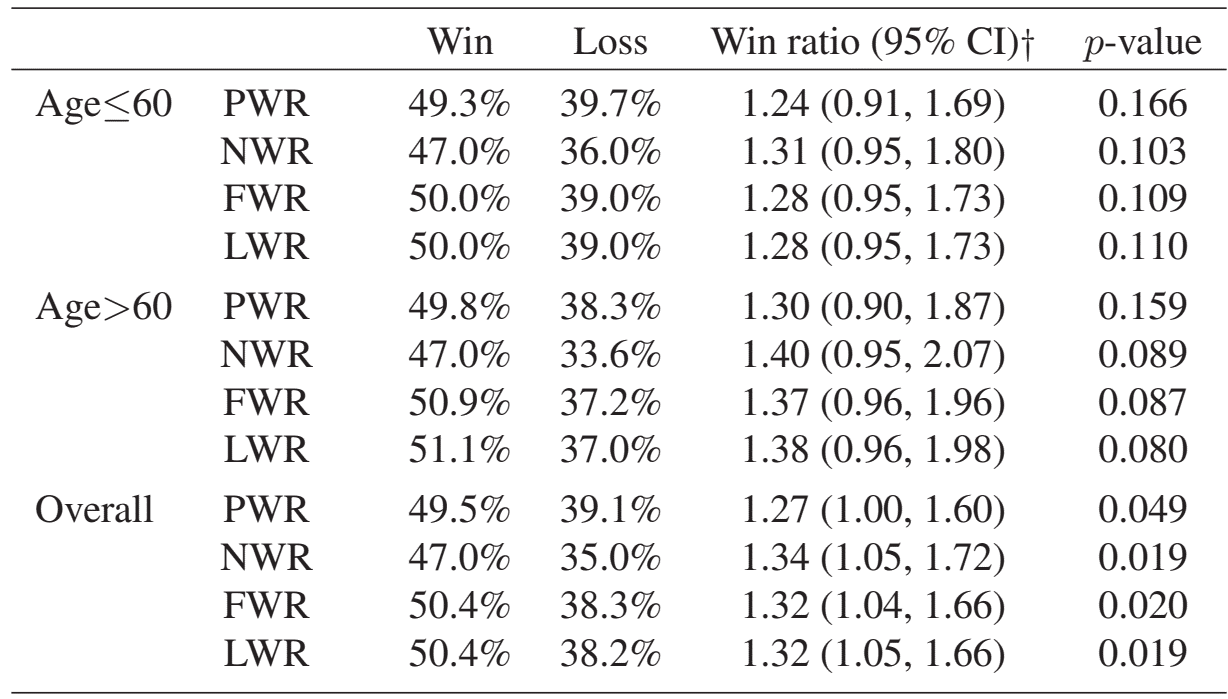
\includegraphics[width=0.7\linewidth,height=\textheight,keepaspectratio]{images/test_hfaction_wr.png}
\end{center}

These results illustrate that recurrent-event WRs detect benefits more
effectively than traditional time-to-first-event WRs, especially when
the number and timing of nonfatal events vary widely across subjects.

\section{Sample Size Calculation}\label{sample-size-calculation}

Sample size calculation for WR is based on a joint model for death and
nonfatal events. Under a Gumbel--Hougaard copula model, the joint
survival function is \[
\pr(D^a > s, T_1^a > t) = \exp\left\{ -\left[ (\lambda_D^a s)^\kappa + (\lambda_H^a t)^\kappa \right]^{1/\kappa} \right\},
\] where \(\lambda_D^a\) and \(\lambda_H^a\) are arm-specific baseline
hazard rates and \(\kappa\) controls the dependence between outcomes.

The required sample size is \[
n = \frac{\zeta_0^2(z_{1-\alpha/2} + z_\gamma)^2}{q(1-q)\delta^\top \xi},
\] where: - \(\zeta_0^2\) is the variance of the test statistic under
the null, - \(\delta\) is the sensitivity of the log-WR to changes in
log-HRs \(\xi\), - \(q\) is the treatment allocation proportion.

Design parameters include the accrual duration \(\tau_b\), total
follow-up time \(\tau\), and a random loss-to-follow-up rate
\(\lambda_L\).

\section{HF-ACTION: Planning a New
Trial}\label{hf-action-planning-a-new-trial}

Using HF-ACTION training arm data as historical reference, the estimated
baseline rates were: - \(\lambda_D = 0.073\) deaths/year -
\(\lambda_H = 0.56\) hospitalizations/year - Kendall's correlation =
36.1\%

Assuming HRs of 0.9 (death) and 0.8 (hospitalization), and minimal loss
to follow-up, the sample size required for 80\% power is approximately
\(n = 1241\).

\begin{center}
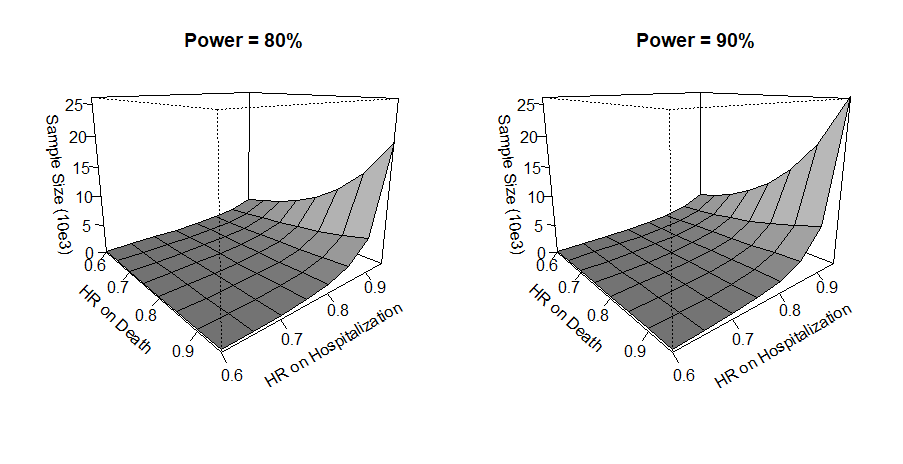
\includegraphics[width=0.9\linewidth,height=\textheight,keepaspectratio]{images/test_hfaction_ss.png}
\end{center}

\section{Example R code}\label{example-r-code}

The following example uses a data frame \texttt{df} in long format with
columns:

\begin{itemize}
\tightlist
\item
  \texttt{id}: subject identifier\\
\item
  \texttt{time}: event or censoring time\\
\item
  \texttt{status}: event type (0 = censoring, 1 = death, 2 = nonfatal)\\
\item
  \texttt{trt}: treatment group (0 = control, 1 = treatment)\\
\item
  \texttt{strata}: optional stratification variable
\end{itemize}

\begin{Shaded}
\begin{Highlighting}[]
\DocumentationTok{\#\#\#\#\#\#\#\#\#\#\#\#\#\#\#\#\#\#\#\#\#\#\#\#\#\#\#\#\#\#\#\#\#\#\#\#\#\#\#\#}
\CommentTok{\# 1. WR test for recurrent events}
\DocumentationTok{\#\#\#\#\#\#\#\#\#\#\#\#\#\#\#\#\#\#\#\#\#\#\#\#\#\#\#\#\#\#\#\#\#\#\#\#\#\#\#\#}
\FunctionTok{library}\NormalTok{(WR)}

\NormalTok{obj }\OtherTok{\textless{}{-}} \FunctionTok{WRrec}\NormalTok{(}\AttributeTok{ID =}\NormalTok{ df}\SpecialCharTok{$}\NormalTok{id, }\AttributeTok{time =}\NormalTok{ df}\SpecialCharTok{$}\NormalTok{time, }\AttributeTok{status =}\NormalTok{ df}\SpecialCharTok{$}\NormalTok{status, }
             \AttributeTok{trt =}\NormalTok{ df}\SpecialCharTok{$}\NormalTok{trt, }\AttributeTok{strata =}\NormalTok{ df}\SpecialCharTok{$}\NormalTok{strata, }\AttributeTok{naive =} \ConstantTok{TRUE}\NormalTok{)}

\CommentTok{\# Extract log win ratio and standard error}
\NormalTok{obj}\SpecialCharTok{$}\NormalTok{log.WR}
\NormalTok{obj}\SpecialCharTok{$}\NormalTok{se}
\FunctionTok{print}\NormalTok{(obj)}
\end{Highlighting}
\end{Shaded}





\end{document}
